\chapter{Evaluation and Analysis of GPU Communication}\label{eval}
This chapter examines anylsis results of the traces generated with the technique described in chapter \ref{chap:impl}.
The analysis will focus on aggregated statistics, rather than averaging. 

\section{Evaluated Applications}
	Set of Functions that can display a communicating behavior, tend to be iterative kernels
\begin{itemize}
	\item Histogram (CUDA Suite)
	\item Stencil (Rodinia 2D, 3D)
	\item NBody (CEG)
	\item BFS (Rodinia)
	\item Pathfinder (Rodinia)
\end{itemize}
%\section{Analysis Parameters}
%\subsection{Communication Classes}
%\begin{itemize}
%	\item P2P: One Writer, one Reader
%	\item Scatter: One Writer, Multiple Readers
%	\item Gather: Multiple Writes, one Reader
%	\item Synchronization: Atomic access to one Address by multiple CTAs
%\end{itemize}
%\subsection{Communication Metrics}
%\begin{itemize}
%	\item Write-to-Read ratio
%	\item Transfer Size Histogram: Data Transferred in one Communication between two CTAs
%	\item Transfer Density: Number of Communications(one Write->Read relation) between CTAs in whole application
%	\item Volume Density: Number of bytes transferred in whole application
%	\item Sparcity: Stride in data Communicated via Scatter/Gather
%\end{itemize}
\section{Tier I Analysis}
\subsection{Communication Fraction}
\begin{figure}[t]
	\centering
	\includegraphics[width=\textwidth]{../../../Global-Memory-Tracing/memtrace-pass/plots/write-com-ratio}
	\caption{Ration of communication to total of all writes.}
	\label{com-ratio}
\end{figure}
\subsection{Density Map}
\begin{figure}
	\begin{subfigure}[b]{0.45\textwidth}
		\includegraphics[width=1\linewidth]{../../../Global-Memory-Tracing/memtrace-pass/plots/heatmap/bfs}
		\caption{BFS}
		\label{fig:density-bfs}
	\end{subfigure}
	\begin{subfigure}[b]{0.45\textwidth}
		\includegraphics[width=1\linewidth]{../../../Global-Memory-Tracing/memtrace-pass/plots/heatmap/hist}
		\caption{Histogram}
		\label{fig:density-hist}
	\end{subfigure}
	\begin{subfigure}[b]{0.45\textwidth}
		\includegraphics[width=1\linewidth]{../../../Global-Memory-Tracing/memtrace-pass/plots/heatmap/hs3d}
		\caption{Hotspot 2D}
		\label{fig:density-hs2d}
	\end{subfigure}
	\begin{subfigure}[b]{0.45\textwidth}
		\includegraphics[width=1\linewidth]{../../../Global-Memory-Tracing/memtrace-pass/plots/heatmap/hs3d}
		\caption{Hotspot 3D}
		\label{fig:density-hs3d}
	\end{subfigure}
	\begin{subfigure}[b]{0.45\textwidth}
		\includegraphics[width=1\linewidth]{../../../Global-Memory-Tracing/memtrace-pass/plots/heatmap/path}
		\caption{Shortest Path}
		\label{fig:density-path}
	\end{subfigure}
	%add desired spacing between images, e. g. ~, \quad, \qquad, \hfill etc. 
	%(or a blank line to force the subfigure onto a new line)
	\hfill
	\begin{subfigure}[b]{0.45\textwidth}
		\includegraphics[width=1\linewidth]{../../../Global-Memory-Tracing/memtrace-pass/plots/heatmap/nbody}
		\caption{NBody}
		\label{fig:density-nbody}
	\end{subfigure}
	\caption{Transfer Density Plots}
	\label{fig:animals}
\end{figure}
\subsection{Volume Map}
\begin{figure}
	\begin{subfigure}[b]{0.45\textwidth}
		\includegraphics[width=1\linewidth]{../../../Global-Memory-Tracing/memtrace-pass/plots/heatmap-vol/bfs}
		\caption{BFS}
		\label{fig:volume-bfs}
	\end{subfigure}
	\begin{subfigure}[b]{0.45\textwidth}
		\includegraphics[width=1\linewidth]{../../../Global-Memory-Tracing/memtrace-pass/plots/heatmap-vol/hist}
		\caption{Histogram}
		\label{fig:volume-hist}
	\end{subfigure}
	\begin{subfigure}[b]{0.45\textwidth}
		\includegraphics[width=1\linewidth]{../../../Global-Memory-Tracing/memtrace-pass/plots/heatmap-vol/hs3d}
		\caption{Hotspot 2D}
		\label{fig:volume-hs2d}
	\end{subfigure}
	\begin{subfigure}[b]{0.45\textwidth}
		\includegraphics[width=1\linewidth]{../../../Global-Memory-Tracing/memtrace-pass/plots/heatmap-vol/hs3d}
		\caption{Hotspot 3D}
		\label{fig:volume-hs3d}
	\end{subfigure}
	\begin{subfigure}[b]{0.45\textwidth}
		\includegraphics[width=1\linewidth]{../../../Global-Memory-Tracing/memtrace-pass/plots/heatmap-vol/path}
		\caption{Shortest Path}
		\label{fig:volume-path}
	\end{subfigure}
	%add desired spacing between images, e. g. ~, \quad, \qquad, \hfill etc. 
	%(or a blank line to force the subfigure onto a new line)
	\hfill
	\begin{subfigure}[b]{0.45\textwidth}
		\includegraphics[width=1\linewidth]{../../../Global-Memory-Tracing/memtrace-pass/plots/heatmap/nbody}
		\caption{NBody}
		\label{fig:volume-nbody}
	\end{subfigure}
	\caption{Transfer Volume Plots}
	\label{fig:animals}
\end{figure}
\subsection{Msg-size Histogram/CDF}
\begin{figure}
	\begin{subfigure}[b]{0.45\textwidth}
		\includegraphics[width=1\linewidth]{../../../Global-Memory-Tracing/memtrace-pass/plots/cdf/bfs}
		\caption{BFS}
		\label{fig:cfd-bfs}
	\end{subfigure}
	\begin{subfigure}[b]{0.45\textwidth}
		\includegraphics[width=1\linewidth]{../../../Global-Memory-Tracing/memtrace-pass/plots/cdf/hist}
		\caption{Histogram}
		\label{fig:density-hist}
	\end{subfigure}
	\begin{subfigure}[b]{0.45\textwidth}
		\includegraphics[width=1\linewidth]{../../../Global-Memory-Tracing/memtrace-pass/plots/cdf/hs2d}
		\caption{Hotspot 2D}
		\label{fig:cfd-hs2d}
	\end{subfigure}
	\begin{subfigure}[b]{0.45\textwidth}
		\includegraphics[width=1\linewidth]{../../../Global-Memory-Tracing/memtrace-pass/plots/cdf/hs3d}
		\caption{Hotspot 3D}
		\label{fig:cfd-hs3d}
	\end{subfigure}
	\begin{subfigure}[b]{0.45\textwidth}
		\includegraphics[width=1\linewidth]{../../../Global-Memory-Tracing/memtrace-pass/plots/cdf/path}
		\caption{Shortest Path}
		\label{fig:cfd-path}
	\end{subfigure}
	%add desired spacing between images, e. g. ~, \quad, \qquad, \hfill etc. 
	%(or a blank line to force the subfigure onto a new line)
	\hfill
	\begin{subfigure}[b]{0.45\textwidth}
		\includegraphics[width=1\linewidth]{../../../Global-Memory-Tracing/memtrace-pass/plots/cdf/nbody}
		\caption{NBody}
		\label{fig:cfd-nbody}
	\end{subfigure}
	\caption{Message Size CFD Plots}
	\label{fig:CDF}
\end{figure}
\subsection{CTA In/Out-Degree}
\begin{figure}
	\begin{subfigure}[b]{0.45\textwidth}
		\includegraphics[width=1\linewidth]{../../../Global-Memory-Tracing/memtrace-pass/plots/com-degree/bfs}
		\caption{BFS}
		\label{fig:deg-bfs}
	\end{subfigure}
	\begin{subfigure}[b]{0.45\textwidth}
		\includegraphics[width=1\linewidth]{../../../Global-Memory-Tracing/memtrace-pass/plots/com-degree/hist}
		\caption{Histogram}
		\label{fig:deg-hist}
	\end{subfigure}
	\begin{subfigure}[b]{0.45\textwidth}
		\includegraphics[width=1\linewidth]{../../../Global-Memory-Tracing/memtrace-pass/plots/com-degree/hs2d}
		\caption{Hotspot 2D}
		\label{fig:deg-hs2d}
	\end{subfigure}
	\begin{subfigure}[b]{0.45\textwidth}
		\includegraphics[width=1\linewidth]{../../../Global-Memory-Tracing/memtrace-pass/plots/com-degree/hs3d}
		\caption{Hotspot 3D}
		\label{fig:deg-hs3d}
	\end{subfigure}
	\begin{subfigure}[b]{0.45\textwidth}
		\includegraphics[width=1\linewidth]{../../../Global-Memory-Tracing/memtrace-pass/plots/com-degree/path}
		\caption{Shortest Path}
		\label{fig:deg-path}
	\end{subfigure}
	%add desired spacing between images, e. g. ~, \quad, \qquad, \hfill etc. 
	%(or a blank line to force the subfigure onto a new line)
	\hfill
	\begin{subfigure}[b]{0.45\textwidth}
		\includegraphics[width=1\linewidth]{../../../Global-Memory-Tracing/memtrace-pass/plots/com-degree/nbody}
		\caption{NBody}
		\label{fig:deg-nbody}
	\end{subfigure}
	\caption{CTA Degree Histogram}
	\label{fig:Cta-degree}
\end{figure}
\subsection{Bisection Volume}
\begin{figure}[t]
	\centering
	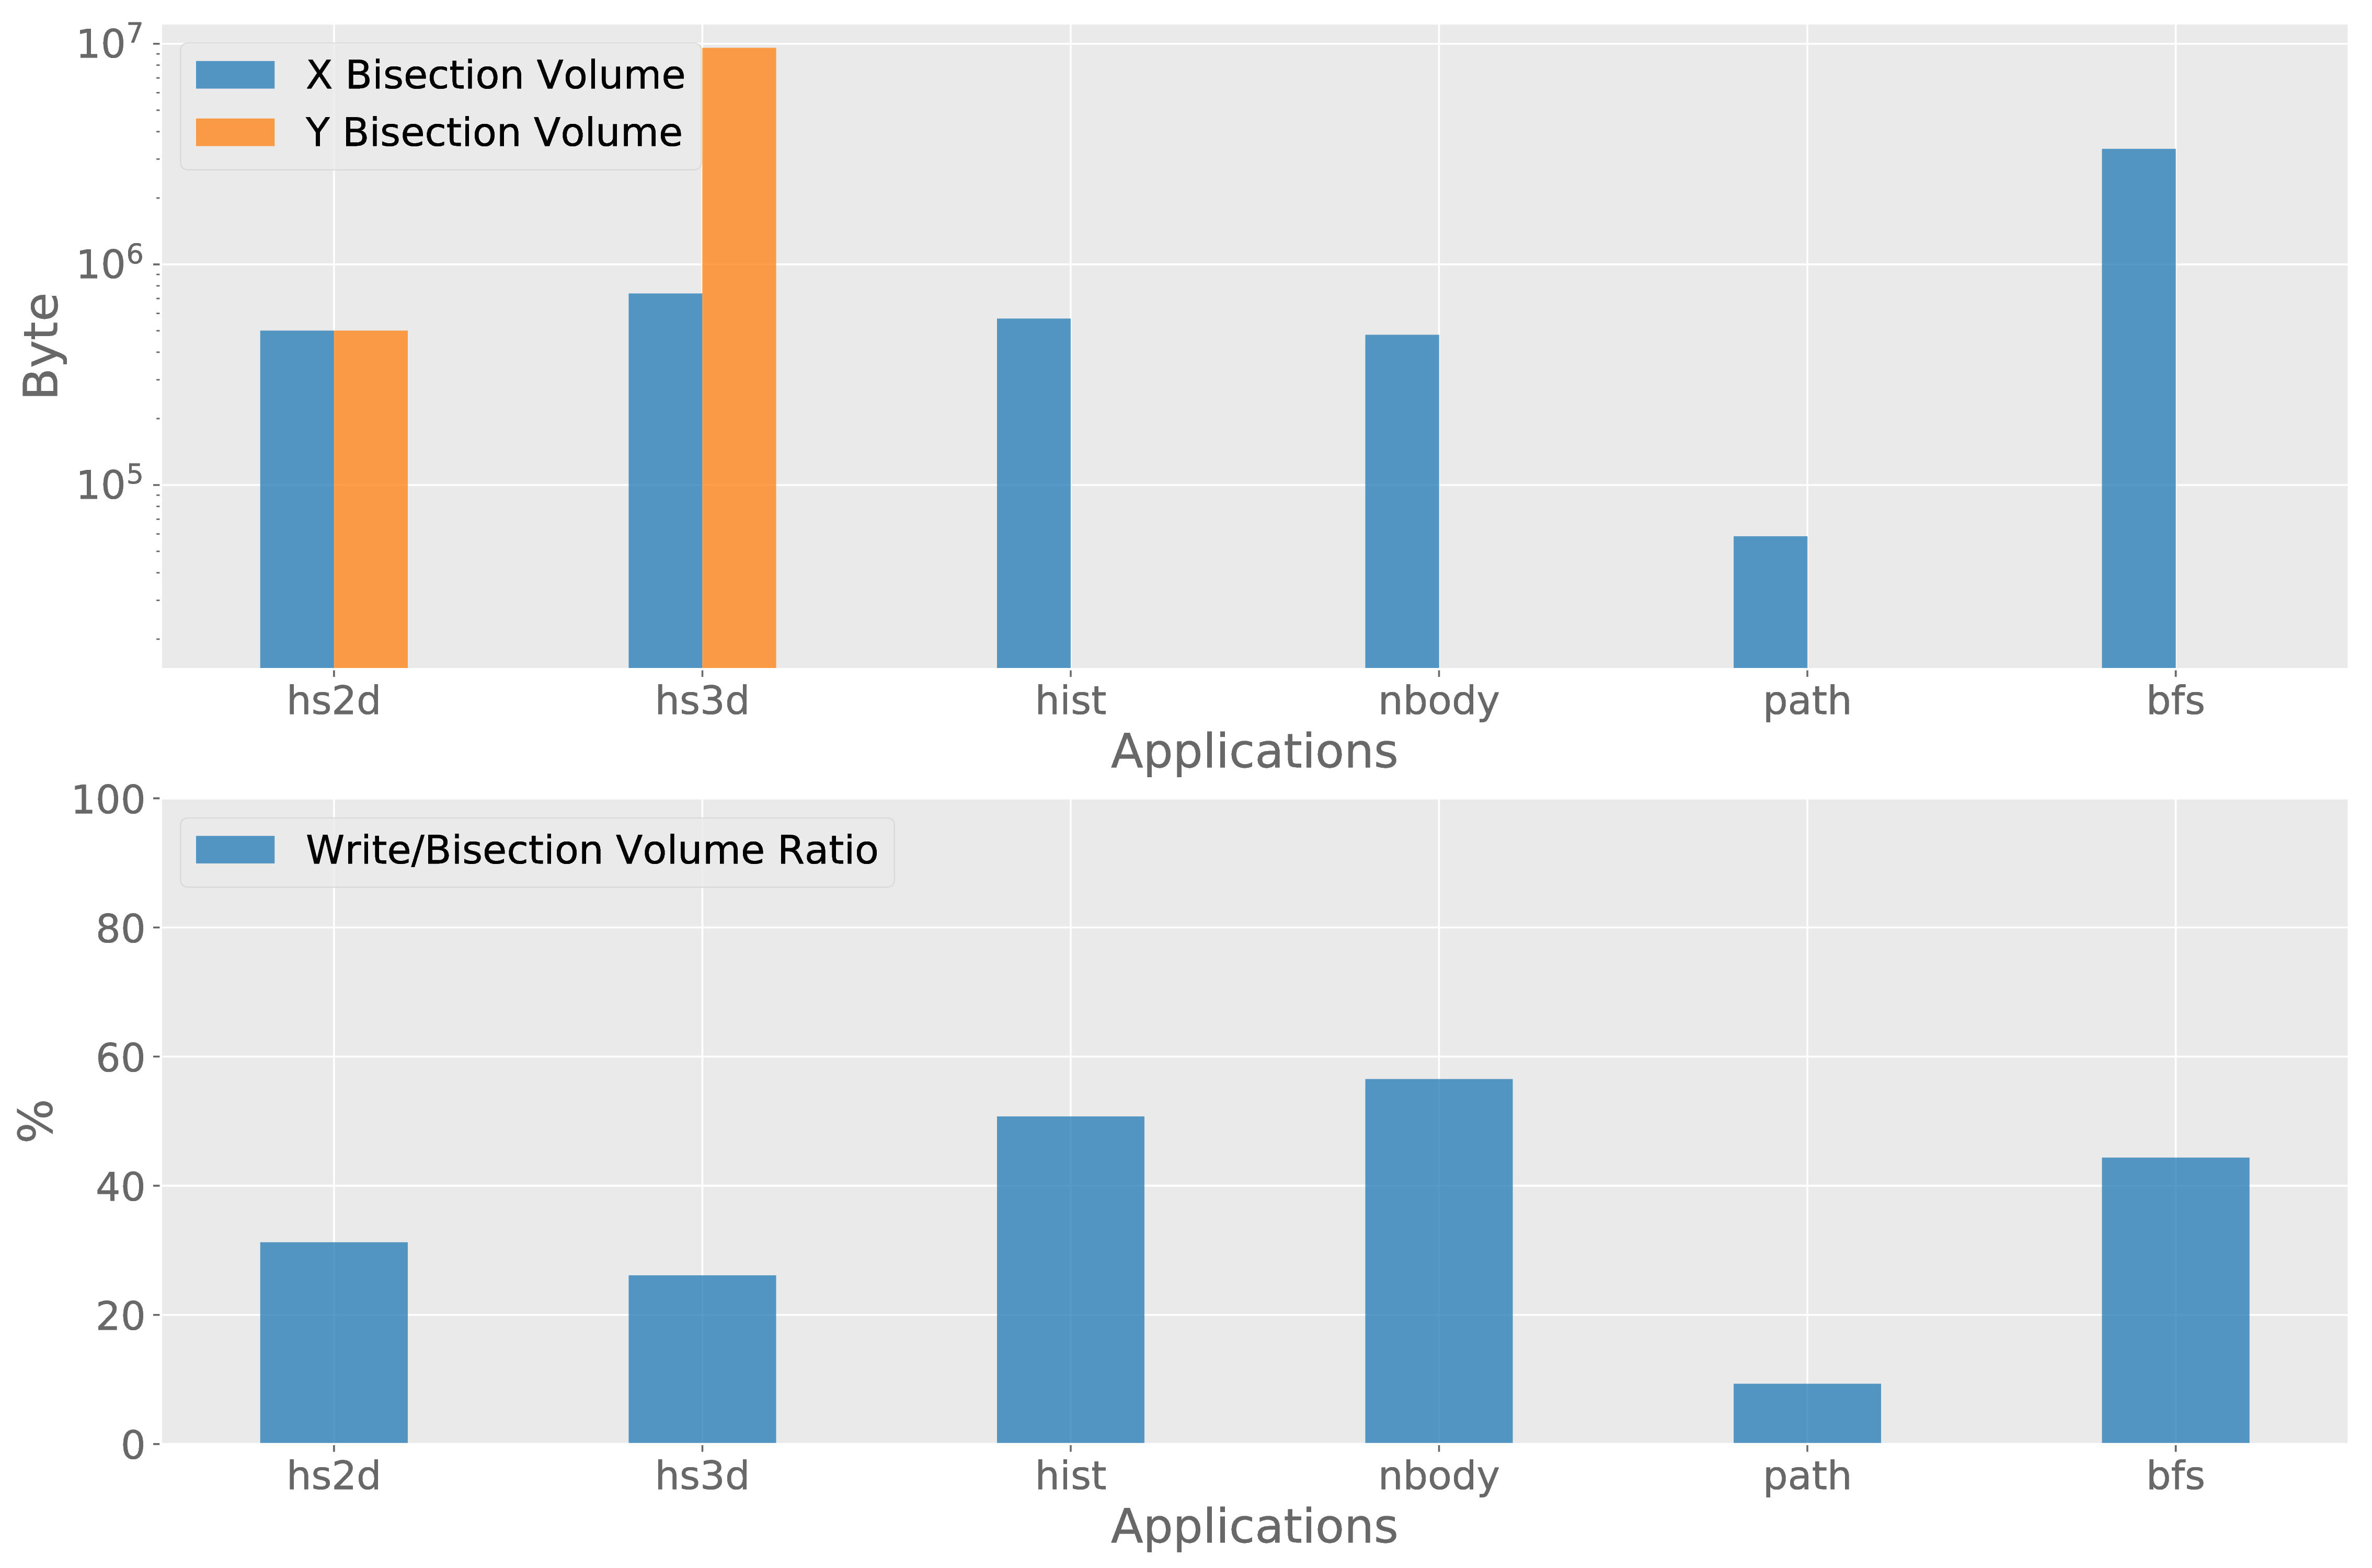
\includegraphics[width=\textwidth]{../../../Global-Memory-Tracing/memtrace-pass/plots/bisection-volume}
	\caption{Bisection Volume}
	\label{bisection-vols}
\end{figure}
\newpage
\section{Tier II Analysis}
\subsection{Kernel communication Evolution}
\begin{figure}[t]
	\centering
	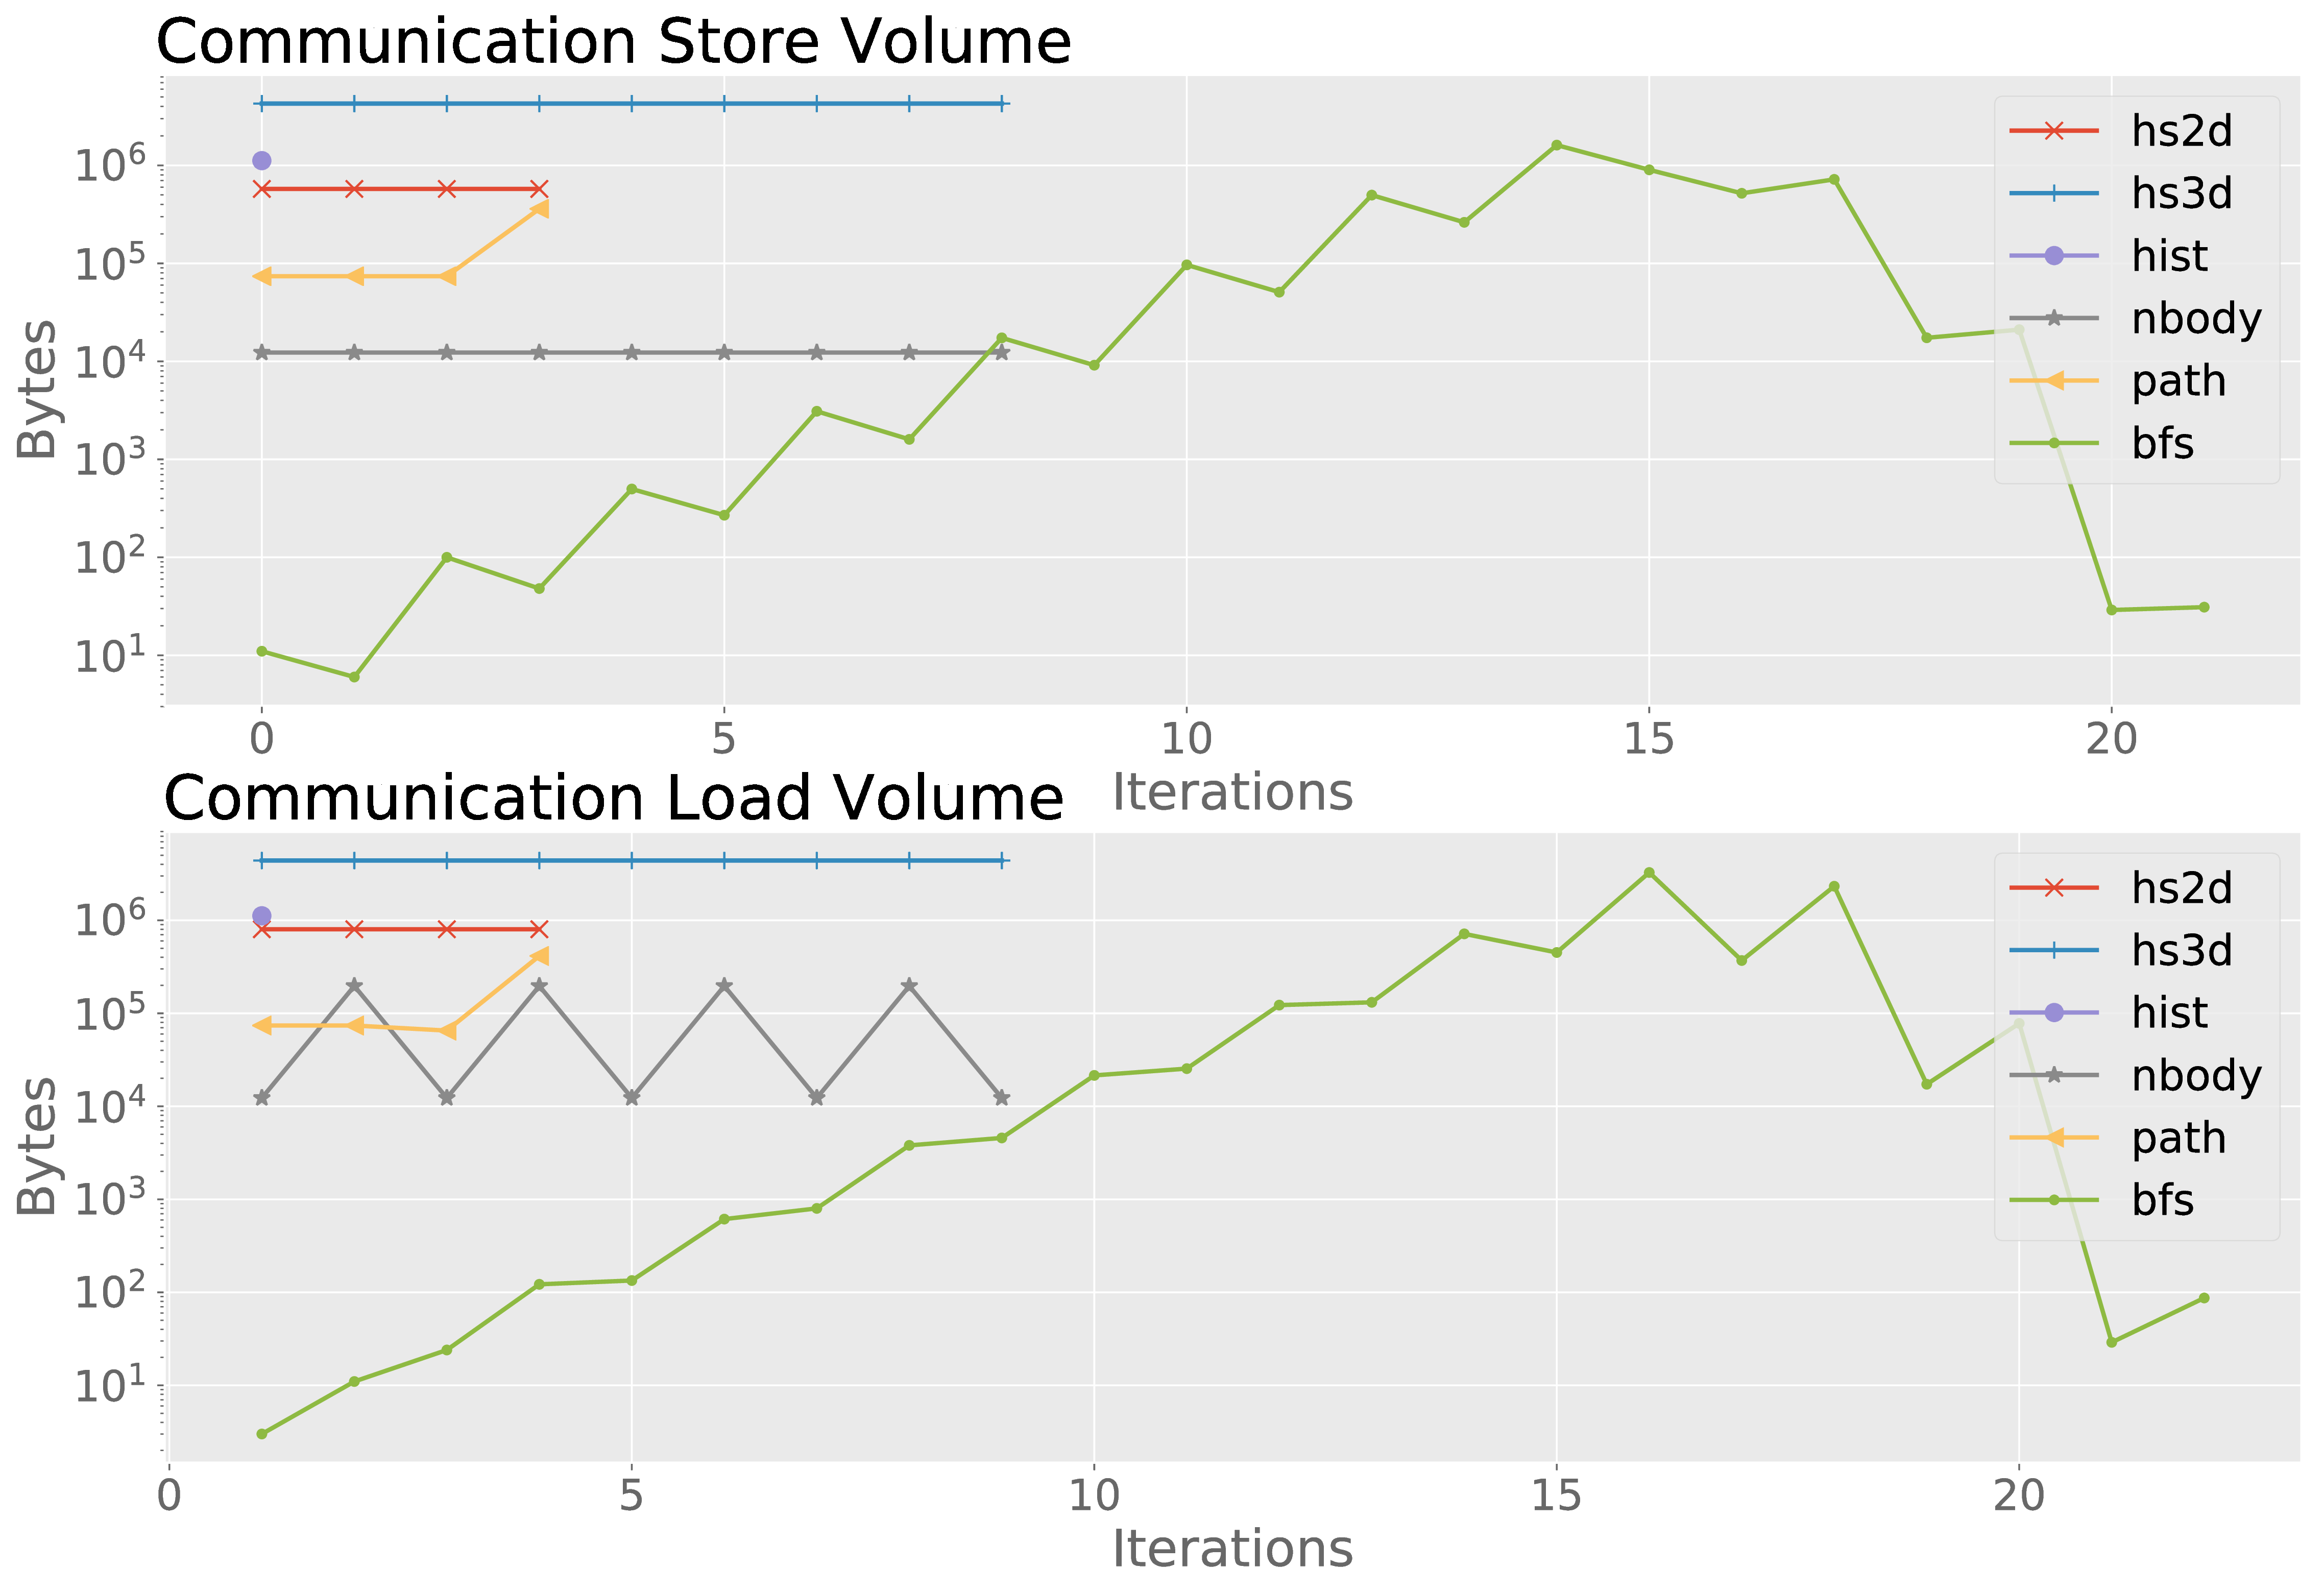
\includegraphics[width=\textwidth]{../../../Global-Memory-Tracing/memtrace-pass/plots/transmission-ratio}
	\caption{Volume of communication writes of each iteration}
	\label{trans-ratio}
\end{figure}
\newpage
\section{Tier III Analysis}
\subsection{Philandering}
%\subsection{Regularity Evolution}
\begin{figure}[t]
	\centering
		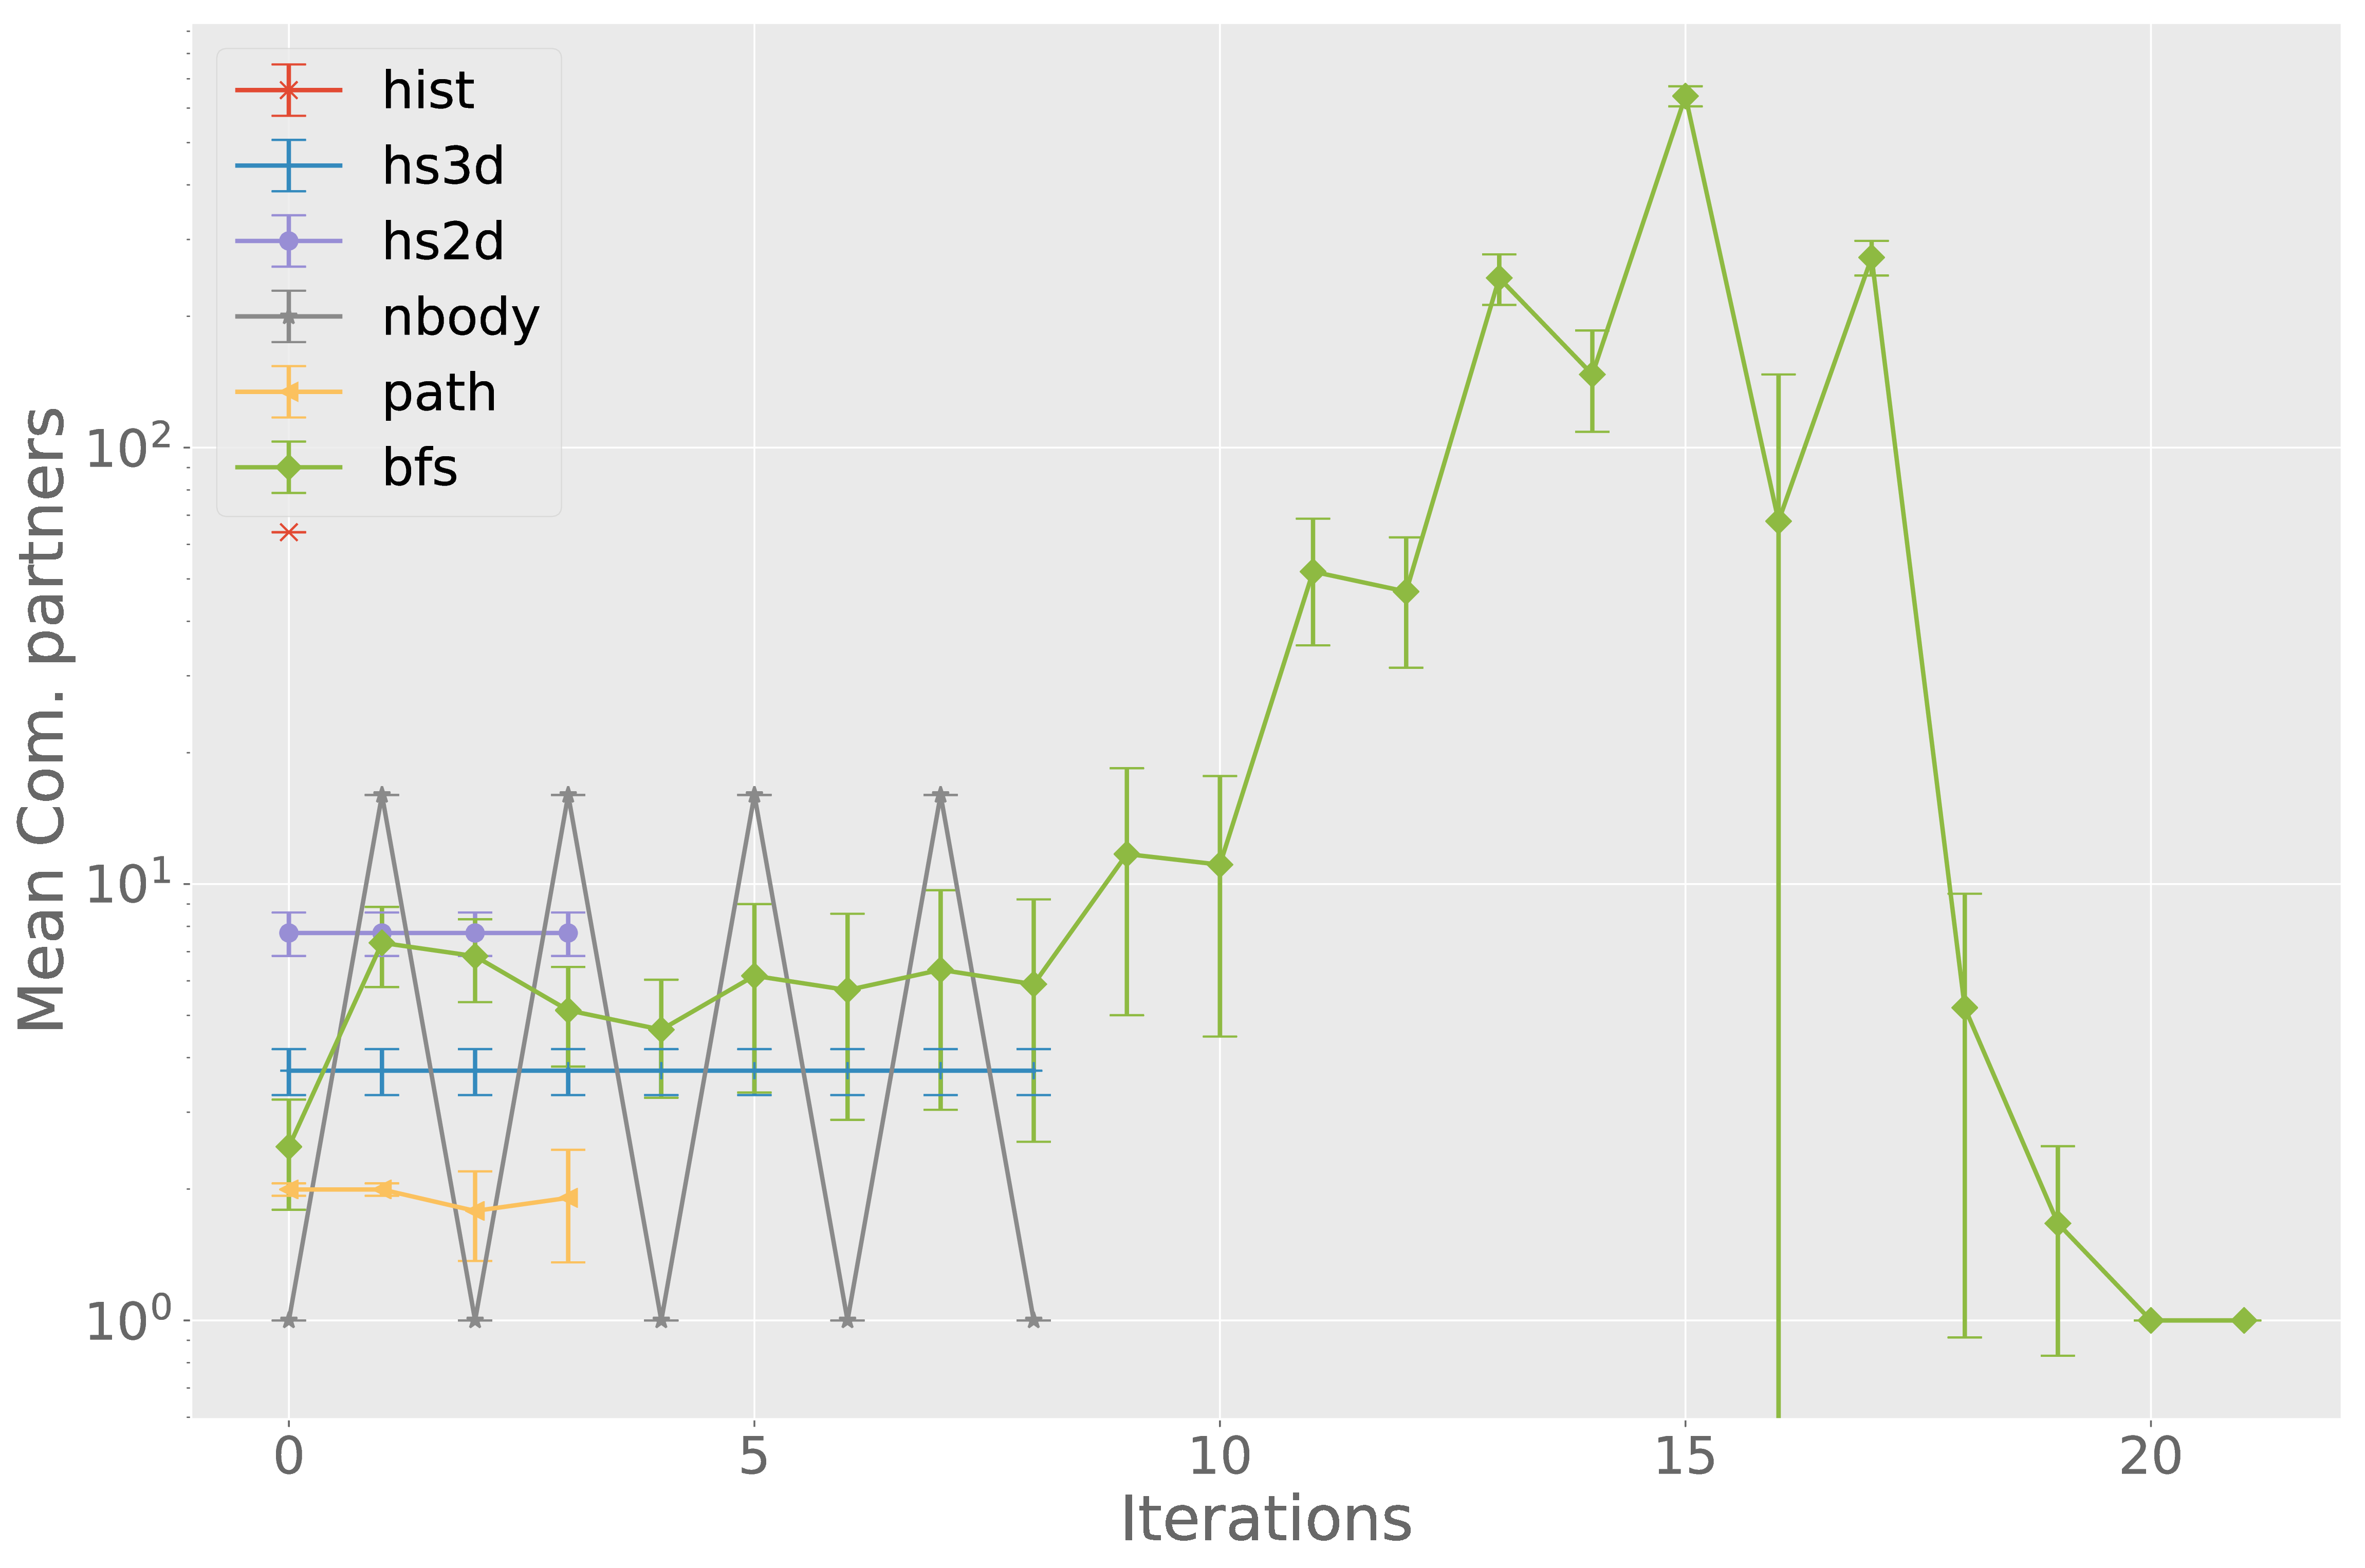
\includegraphics[width=\textwidth]{../../../Global-Memory-Tracing/memtrace-pass/plots/transmission-regularity}
	\caption{Regularity of CTA communication, per iteration partners}
	\label{trans-ratio}
\end{figure}